% interactcadsample.tex
% v1.03 - April 2017

\documentclass[]{interact}

\usepackage{epstopdf}% To incorporate .eps illustrations using PDFLaTeX, etc.
\usepackage{subfigure}% Support for small, `sub' figures and tables
%\usepackage[nolists,tablesfirst]{endfloat}% To `separate' figures and tables from text if required

\usepackage{natbib}% Citation support using natbib.sty
\bibpunct[, ]{(}{)}{;}{a}{}{,}% Citation support using natbib.sty
\renewcommand\bibfont{\fontsize{10}{12}\selectfont}% Bibliography support using natbib.sty

\theoremstyle{plain}% Theorem-like structures provided by amsthm.sty
\newtheorem{theorem}{Theorem}[section]
\newtheorem{lemma}[theorem]{Lemma}
\newtheorem{corollary}[theorem]{Corollary}
\newtheorem{proposition}[theorem]{Proposition}

\theoremstyle{definition}
\newtheorem{definition}[theorem]{Definition}
\newtheorem{example}[theorem]{Example}

\theoremstyle{remark}
\newtheorem{remark}{Remark}
\newtheorem{notation}{Notation}


% tightlist command for lists without linebreak
\providecommand{\tightlist}{%
  \setlength{\itemsep}{0pt}\setlength{\parskip}{0pt}}



\usepackage{hyperref}
\usepackage{tikz-dependency}
\usepackage[utf8]{inputenc}
\usepackage{array}
\usepackage{threeparttable}
\usepackage[final]{changes}
\def\tightlist{}

\usepackage{booktabs}
\usepackage{longtable}
\usepackage{array}
\usepackage{multirow}
\usepackage{wrapfig}
\usepackage{float}
\usepackage{colortbl}
\usepackage{pdflscape}
\usepackage{tabu}
\usepackage{threeparttable}
\usepackage{threeparttablex}
\usepackage[normalem]{ulem}
\usepackage{makecell}
\usepackage{xcolor}

\begin{document}


\articletype{ARTICLE TEMPLATE}

\title{Transformer based named entity recognition for place name
extraction from unstructured text}


\author{\name{Cillian Berragan$^{a}$, Alex Singleton$^{a}$, Alessia
Calafiore$^{b}$, Jeremy Morley$^{c}$}
\affil{$^{a}$Geography and Planning, University of
Liverpool; $^{b}$Edinburgh College of Art, University of
Edinburgh; $^{c}$Ordnance Survey}
}

\thanks{CONTACT Cillian
Berragan. Email: \href{mailto:c.berragan@liverpool.ac.uk}{\nolinkurl{c.berragan@liverpool.ac.uk}}, Alex
Singleton. Email: \href{mailto:alex.singleton@liverpool.ac.uk}{\nolinkurl{alex.singleton@liverpool.ac.uk}}, Alessia
Calafiore. Email: \href{mailto:acalafio@ed.ac.uk}{\nolinkurl{acalafio@ed.ac.uk}}, Jeremy
Morley. Email: \href{mailto:Jeremy.Morley@os.uk}{\nolinkurl{Jeremy.Morley@os.uk}}}

\maketitle

\begin{abstract}
Place names embedded in online natural language text present a useful
source of geographic information. Despite this, many methods for the
extraction of place names from text use pre-trained models that were not
explicitly designed for this task. Our paper builds five custom-built
Named Entity Recognition (NER) models, and evaluates them against three
popular pre-built models for place name extraction. The models are
evaluated using a set of manually annotated Wikipedia articles with
reference to the F\textsubscript{1} score metric. Our best performing
model achieves an F\textsubscript{1} score of 0.939 compared with 0.730
for the best performing pre-built model. Our model is then used to
extract all place names from Wikipedia articles in Great Britain,
demonstrating the ability to more accurately capture unknown place names
from volunteered sources of online geographic information.
\end{abstract}

\begin{keywords}
Named entity recognition; volunteered geographic information; natural
language processing; place name extraction
\end{keywords}

\hypertarget{introduction}{%
\section{Introduction}\label{introduction}}

Place names are frequently encountered in natural language and provide
an additional geographic dimension to much of the textual information
present online, when associated with spatial coordinates and geographic
locations. Despite this, research in place name extraction primarily
concentrates on entities as described by annotation schemes that do not
explicitly consider geographic place names
\citep{karimzadeh2019, halterman2017, hu2019}. Pre-built named entity
recognition (NER) models based on these schemes are also not task
specific; trained on data unrelated to the task they are used for,
despite language involving place names varying significantly depending
on the context \citep{purves2018}. When identifying place names in text,
research typically only considers known administrative names and their
associated strict boundaries, despite natural language often containing
place names that either do not exist formally, are hyper-localised
e.g.~street names, or are alternative names that may be absent from
administrative databases, which often only consider a single formal
name.

The training corpora used by pre-built NER models typically identifies a
number of entities that have no relevance to geographic place names,
e.g.~persons, and those that have some relevance in specific contexts;
locations, geopolitical entities or facilities
\citep{weischedelralph2013, tjongkimsang2003}. Notably, they do not
specifically target a `place name' entity, meaning, while often these
three related entity types may often refer to a place name, this is not
always the case. Additionally, these corpora consist of text that often
differs in structure, compared with the text being processed by models
trained using them; for example social media text is typically more
informal compared with the news articles used to build the popular
dataset, CoNLL03 \citep{tjongkimsang2003}.

New forms of geographic information online present an opportunity to
train and evaluate models on texts that contain a large volume of place
names \citep{goodchild2011}, building models from the ground up, and
using annotation schemes that are explicitly designed for the extraction
of place names from text. Results from these models are expected to
outperform existing pre-built models which use unrelated training data,
and do not include a `place name' entity type.

Our paper presents five NER models, trained on manually labelled
Wikipedia data and used to identify and extract any span of text
considered to be a place name, from articles relating to geographic
locations in the United Kingdom. Our model is evaluated against
pre-built solutions that are commonly used for this task, demonstrating
the importance of model training with task specific data, and the
consideration that named entity recognition as a task is not appropriate
for place name extraction, due to the exclusion of a `place name' entity
type, and the inclusion of a number of unrelated entities. New
developments in natural language processing (NLP) are utilised,
outlining the benefit of selecting modern architectures that are not yet
implemented by off the shelf models. Our paper considers the ability to
extract place names from Wikipedia articles for the United Kingdom that
do not appear in the GeoNames Gazetteer, with the goal of identifying
the additional geographic information that may be effectively extracted
from unstructured sources of online text.

Section \ref{literature-review} outlines the research and concepts
associated with geography in NLP, considering its relation to the new
forms of geographic data present online, the techniques in natural
language processing that explicitly deal with geography, and the
developments in NLP that have enabled higher accuracy with limited
labelled data. Section \ref{methodology} presents the workflow
undertaken for the models constructed in this paper, as well as the data
collection and analysis of the entities extracted.

The performance of each NER model is then presented in Section
\ref{results-discussion} and evaluated against pre-built solutions using
a corpus of labelled test data. Place names are extracted using the
model for the entire Wikipedia corpus, and compared against GeoNames,
identifying names that are not present, discussing the reasons they may
be found within Wikipedia articles, but not in an explicitly geographic
gazetteer.

\hypertarget{literature-review}{%
\section{Literature review}\label{literature-review}}

Natural language often describes places using imprecise referents,
non-administrative names, and an understanding of place footprints that
does not conform with the formal administrative boundaries given to them
\citep{gao2017, goodchild2011}. Despite this, regions and place names in
computational geography are usually formally defined by administrative
datasets, meaning any informal place names are unable to be identified,
or associated with a position in space. This distinction has given rise
to a focus on \emph{place} based GIS, rather than \emph{space} based,
which considers the ability to capture place references that may not
appear in administrative datasets \citep{gao2013}.

Since the advent of Web 2.0, increased access to mobile devices which
include passive GPS and open-access mapping information, several
scientific disciplines have developed to take advantage of the data
being produced, including crowdsourcing, and user-generated content
\citep{see2016}. With geographically referenced content through social
media, mapping platforms and Wikipedia there is now a wealth of
information that \citet{goodchild2007} terms \emph{`Volunteered
Geographic Information'} (VGI). These data sources present a large
collection of continually updated references to places, often providing
informal and unstructured geographic information.

Much of the past work using VGI has concentrated either on explicitly
geographic crowd-sourced mapping platforms like Open Street Map
\citep{antoniou2010}, or `geotagged' content which enables, often
passively contributed, user-generated data through sites like Twitter or
Flickr, used to extract geographic information. \citet{gao2017} for
example present an approach for the construction of cognitive regions
from various VGI sources, querying place names found in tags with
associated geotags to create vague boundaries. A similar approach is
taken by \citet{hollenstein2010} who identified tags containing vague
spatial concepts like `downtown' and `citycentre', deriving regions from
geotags. These methods demonstrate the ability to derive informal
geographic information from VGI, while giving similar results to that of
manually collected questionnaire data \citep{twaroch2019, gao2017}.

While this work concentrates solely on the use of geotags and short
single phrase tags associated with social media documents to analyse
`place' focussed geographies, another source of online information that
is less frequently considered to have geographic properties is
unstructured text, which has the potential to provide an even larger
source of geographically focussed information. Good results have been
reported using basic semantic rules to identify places names found in
unstructured text \citep{moncla2014}, however, these methods have relied
on this text almost solely containing place names as entities.
Alternatively to rule-based approaches, \citet{hu2019} demonstrate the
use of four pre-trained NER models to extract local, informal place
names from housing advertisements descriptions with associated
coordinates, to enrich existing gazetteers with place names not normally
present, alongside derived boundaries. The results of this paper show
the promising ability for NER models to extract informal place names
directly from text, also demonstrating a bottom-up approach to gazetteer
construction, enabling informal place definitions to be captured from
VGI, that may be absent from administrative datasets. Model evaluation
however showed low precision and recall when evaluating against a
labelled dataset, reflecting issues with the use of pre-built NER models
for this task. Similar evaluation results are observed by
\citet{karimzadeh2019} when considering various pre-built NER models for
use in the GeoTxt geoparsing system, which uses either SpaCy or Stanza
pre-built models \citep{qi2018, honnibal2017}. While the precision of
these pre-built NER models can be relatively high for more sophisticated
models, they all suffer from low recall. \citet{karimzadeh2019} note
particularly that while improved results would be expected by training a
model from the ground up, the amount of labelled training data required
to create a suitable model would be very large. To improve the accuracy
of systems that rely on place name extraction, NER models should be
constructed with more suitable training data, and with annotations
tailored for this specific task.

While large, open-access, text-based sources of semantic geographic
information are scarce, Wikipedia provides a large collection of
articles about almost any subject, many of which relate to geographic
locations. This presents an alternative data source for use in
geographically focussed NLP applications, with place names, their
semantic context, and article geotags providing geographic information.
Various studies have used Wikipedia as a data source for the extraction
of place names, \citet{delozier2015} for example, identify place names
in Wikipedia articles and use a clustering technique using document
contexts to disambiguate their geographic locations.
\citet{speriosu2013} use geotagged Wikipedia articles to provide
contextual information regarding a range of place names for
disambiguation. Both these works first use a pre-built Named Entity
Recognition (NER) model to identify place names found in text, before
further analysis. Improvements made to these NER models for place name
extraction present a stronger foundation, leading to both better recall,
and precision of place names being identified, before they are resolved
to coordinates \citep{leidner2008, purves2018}. Our paper selects
Wikipedia articles to demonstrate the geographic information that may be
extracted from unstructured text, presenting a first-stage baseline
approach for tasks that rely on accurate place name extraction.

\hypertarget{named-entity-recognition-in-the-geographic-domain}{%
\subsection{Named entity recognition in the geographic
domain}\label{named-entity-recognition-in-the-geographic-domain}}

Natural language processing techniques involving geography typically
focus around geoparsing; the automated extraction of place names from
text, followed by the resolution of the identified place names to
geographic coordinates \citep{gritta2020, leidner2008, buscaldi2011}.
Modern place name extraction techniques primarily rely on named entity
recognition (NER) to identify place names as entities within text
\citep{kumar2019, purves2018}. While most pre-built NER systems are able
to identify `geopolitical entities' and `locations' as defined by
popular annotation schemes\footnote{CoNLL03:
  \url{https://www.clips.uantwerpen.be/conll2003/ner/}, OntoNotes 5:
  \url{https://catalog.ldc.upenn.edu/LDC2013T19}}, these only act as a
proxy for place names in text. The majority of entities recognised by
these systems are unrelated to place names, and as such simply
contribute to lower overall recall when other entities are preferred by
models over geographic place names. For example, a model may consider a
named organisational headquarters as an `organisation' entity, rather
than a `location', even when used as a locational reference.

The concept of a place name as an entity defined by the labelled corpora
NER models were trained on hinders place name extraction, identifying
only (and any) administrative place names in text \citep{gritta2017a}.
The geoparser \emph{Mordecai}\footnote{\url{https://github.com/openeventdata/mordecai}}
for example, uses an NER tagger provided through the \texttt{SpaCy}
Python library, which provides a variety of entities including those
unrelated to place names (e.g.~\textbf{PER}: persons), and three
entities that may be considered related, \textbf{GPE} (Geopolitical
Entity), \textbf{LOC} (Location), and \textbf{FAC} (Facility). While
these categories often do relate to place names, they do not consider
whether the entity could be contextually considered a place name that
could be geo-located. For example, geopolitical entities are often used
in a metonymic sense; a figure of speech where a concept is substituted
by a related concept. In the phrase `Madrid plays Kiev today' for
example, sports teams are replaced by their associated place name
\citep{gritta2020}. As place name based metonyms do not explicitly
relate to geographic locations, and instead a related entity, we are
uninterested in their extraction. Due to the reliance on large labelled
corpora for NER training, and limited source of geography specific data
\citep{karimzadeh2019}, little work has considered explicitly targeting
place names through new data, as it is often time-consuming to produce.

While at present pre-built NER models identify entities as defined by
widely used annotated corpora, some work has considered the need to
identify \emph{spatial} entities. SpatialML is a natural language
annotation scheme that presents the \textbf{PLACE} tag for any mention
of a location \citep{mani2010}. Tasks identified by the
\href{https://semeval.github.io/}{Semantic Evaluation Workshop} built on
this annotation scheme and defined several entities relating to spatial
language \citep[SemEval-2015 Task 8: SpaceEval,][]{pustejovsky2015},
described by the ISO-Space annotation specification
\citep{pustejovsky2017}. In order to more appropriately consider
geography when parsing unstructured text for place related entities,
models should be built from the ground up, taking into account an
alternative annotation scheme that identifies place names, excluding
unrelated entities.

Recent progress in NLP and the use of GPU accelerated training has
brought with it the ability to process large quantities of unlabelled
text. This development has recently led to the creation of general
purpose `language models' that implement the `transformer' architecture,
using semi-supervised learning to train using very large corpora
\citep{vaswani2017}. For example, Google's pioneering BERT model was
trained using the entirety of English Wikipedia, and over 11,000 books
\citep{devlin2019}. This development has led to models which perform
well for many given tasks, even with relatively limited additional
labelled training data.

Our paper proposes fine-tuning transformer-based language models for
place name extraction using named entity recognition, to extract all
place names from UK `place' classed articles on Wikipedia. 200 of these
articles are annotated, labelling place names to train and evaluate
model performance. We train and compare the performance of three popular
transformer-based NER models; BERT - a large, popular transformer model,
RoBERTa - similar to BERT, using a different pre-training procedure,
which has had better results on some tasks, and DistilBERT - a much
smaller and less complex transformer model based on RoBERTa. In addition
to these transformer models, two simpler Bidirectional LSTM (BiLSTM)
models are compared, one using pre-trained GloVe embeddings,
representing an equivalent complexity model used by Stanza or SpaCy
pre-built NER solutions, and another showing a baseline model without
any pre-trained word embeddings. These models are then evaluated against
three pre-built NER systems that are popular for place name extraction,
and used in existing geoparsing systems including GeoTxt and Mordecai.

\hypertarget{methodology}{%
\section{Methodology}\label{methodology}}

Figure \ref{fig:workflow} gives an overview of the model and data
processing pipeline used in our paper. This section first outlines the
computational infrastructure used. The data collection and data
processing is then described, obtaining a corpus of Wikipedia articles
for locations in Great Britain with place names labelled.

This dataset was then used to train custom NER models of various
architectures, which were evaluated using separate test data against
each other and popular pre-built NER models. We then selected our
DistilBERT transformer model to extract all place names from the full
corpus of Wikipedia articles, as this model performed well as indicated
by its test F\textsubscript{1} score, despite its smaller size.

\begin{figure}[tb]

{\centering 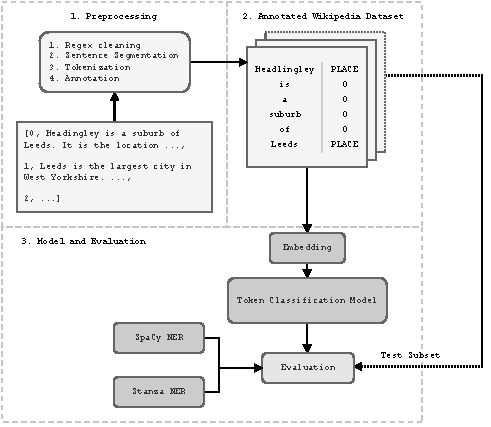
\includegraphics[width=\linewidth]{figures/figure1_template} 

}

\caption{Overview of the model processing pipeline}\label{fig:workflow}
\end{figure}

\hypertarget{software-hardware-infrastructure}{%
\subsection{Software \& hardware
infrastructure}\label{software-hardware-infrastructure}}

Models used in our paper were written in
\href{https://www.python.org/}{\texttt{Python}} using the
\href{https://allennlp.org/}{\texttt{AllenNLP}} library for deep
learning in natural language processing \citep{gardner2018}.
\texttt{AllenNLP} is built on top of
\href{https://pytorch.org}{\texttt{PyTorch}} \citep{paszke2019},
providing abstractions to commonly used operations for working with
state-of-the-art deep neural networks in natural language processing.

Model training was GPU accelerated using a single NVIDIA GeForce RTX
2070 SUPER with 8192MB memory paired with a Ryzen 3700x CPU with 8
physical and 16 logical cores. \texttt{Python} version 3.8.5 was used
with \texttt{AllenNLP} version 1.5.0.

\hypertarget{annotation-data-collection}{%
\subsection{Annotation \& data
collection}\label{annotation-data-collection}}

\hypertarget{wikipedia-data-collection}{%
\subsubsection{Wikipedia data
collection}\label{wikipedia-data-collection}}

Wikipedia presents a large collection of well-formatted text contributed
by a variety of users, with frequent instances of place names, a
consistent written style and without misspellings. Existing NER models
are trained on either CoNLL-03 or OntoNotes 5, both of which are
well-formatted text datasets, consisting primarily of news articles. As
such, it was considered appropriate to select Wikipedia for a comparison
between these models and ours, compared with other sources of VGI that
are of lower overall quality.

The Wikipedia text data used in our paper was accessed through
\href{https://wiki.dbpedia.org/}{DBpedia} \citep{auer2007}, a community
gathered database of information from Wikipedia, presented as an open
knowledge graph, with ontologies that link and define information in
articles. A query was built to obtain English Wikipedia abstracts for
each DBpedia article with the \texttt{Place} class in Great Britain,
using the \href{http://dbpedia.org/sparql}{DBpedia SPARQL endpoint}.
Querying just for \texttt{Place} articles within Great Britain ensured
that articles extracted contained a large number of place names and
language indicative of place names, without additional, unnecessary
information.

These abstracts are the text provided at the top of each article, before
any headings, sometimes called the summary. As an example, the Wikipedia
abstract for \href{https://en.wikipedia.org/wiki/Rowlatts_Hill}{Rowlatts
Hill}, a suburb of Leicester, UK is as follows, with hyperlinks
indicated in bold:

\begin{quote}
Rowlatts Hill (also known as Rowlatts Hill Estate, or R.H.E.) is an
eastern, residential suburb of the \textbf{English} city of
\textbf{Leicester}. It contains mostly \textbf{council-owned housing}.
\end{quote}

\begin{quote}
The suburb is roughly bordered by Spencefield Lane to the east and
Whitehall Road to the south, which separates it from neighbouring
\textbf{Evington}. A second boundary within the estate consists of
Coleman Road to Ambassador Road through to Green Lane Road; Rowlatts
Hill borders \textbf{Crown Hills} to the west. To the north, at the
bottom of Rowlatts Hill is Humberstone Park which is located within
Green Lane Road, Ambassador Road and also leads on to Uppingham Road
(the \textbf{A47}), which is also Rowlatts Hill.
\end{quote}

Using DBpedia enabled a fast executing query which, when combined with
the \texttt{Place} class from the DBpedia ontology, returned a complete
dataset of Wikipedia pages for many geographic locations in Great
Britain. A total 42,222 article abstracts were extracted.

\hypertarget{input-format}{%
\subsubsection{Input format}\label{input-format}}

For use in the models, a random subset of 200 articles were annotated
using the CoNLL-03 NER format, which uses line delimitation to separate
tokens, with entities associated with each token sharing the same line,
separated by a space. Articles were first cleaned using regular
expressions to remove quotation marks, text inside parentheses, and
non-ascii characters. The \texttt{SpaCy} large web-based pre-trained
model pipeline (\texttt{en\_core\_web\_lg}) was used for further
processing, using a non-monotonic arc-eager transition-system for
sentence segmentation \citep{honnibal2015}, and tokenisation using a
rule-based algorithm. Each sentence-length sequence of tokens was
treated as a separate instance to be fed as batches into models for
training. Each token in every sequence was annotated as being a place
name or not, assisted through the open source annotation tool
\href{https://github.com/doccano/doccano}{Doccano} \citep{nakayama2018}.

For place names that span multiple tokens, the \emph{BIOUL} tagging
scheme was used, which stands for the `\emph{\textbf{B}eginning},
\emph{\textbf{I}nside} and \emph{\textbf{L}ast} tokens of multi-token
chunks'; for place names that span more than one token
(e.g.~\emph{B-Place}: New, \emph{L-Place}: York).
`\emph{\textbf{U}nit-length} chunks and \emph{\textbf{O}utside}', place
names of only a single token, and outside for any token that isn't a
place name. This scheme was used over the simpler BIO scheme which is
more difficult for models to learn \citep{ratinov2009}. During
annotation it became clear that the length of certain multi-token place
names could be considered ambiguous. For example, it may not be clear
when a cardinal direction is part of a place name, `northern Ireland'
may refer to a northern region in Ireland, while `Northern Ireland'
refers to the constituent country in the United Kingdom. To unify
labelling decisions we chose to consider capitalisation as an indication
of multi-token noun phrases that constituted a single place name. The
following sentence shows a sequence of tokens with their corresponding
tags, demonstrating the annotation scheme with \emph{BIOUL} information
prepending each tag:

\begin{figure}[H]
\centering
\begin{dependency}
\tikzstyle{word}=[font=\normalsize]
\tikzstyle{tag}=[font=\bfseries\tiny]
\begin{deptext}[column sep=0.05cm, row sep=0.1cm]
\& |[word]| \textit{Kingston} \& |[word]| \textit{upon} \& |[word]| \textit{Hull} \& |[word]| is
\& |[word]| usually \& |[word]| abbreviated  \& |[word]| to \& |[word]| \textit{Hull} \\
\& |[tag]| B-PLACE \& |[tag]| I-PLACE \& |[tag]| L-PLACE \& |[tag]| O
\& |[tag]| O \& |[tag]| O \& |[tag]| O \& |[tag]| U-PLACE \\
\end{deptext}
\end{dependency}
\end{figure}

From these 200 labelled Wikipedia abstracts, 10\% were kept for both
validation and testing, leading to a training set of 21,080 labelled
tokens, a validation dataset of 2,907 labelled tokens, and a testing
dataset of 3,347 labelled tokens.

\hypertarget{building-the-entity-recognition-models}{%
\subsection{Building the entity recognition
models}\label{building-the-entity-recognition-models}}

Named entity recognition is a subset of token classification where a
sequence of tokens \(\mathbf{x} = \{x_{0}, x_{1}\dots x_{n}\}\) are
taken as input, and the most likely sequence tags
\(\mathbf{y} = \{y_0, y_1, \dots y_n\}\) are predicted. The models
constructed in our paper may be divided into three main components,
outlined on Figure \ref{fig:workflow}:

\begin{itemize}
\tightlist
\item
  \textbf{Embedding Layer}: Each token in a sequence represented as high
  dimension numerical space, they may be either:

  \begin{itemize}
  \tightlist
  \item
    Randomly initialised
  \item
    Pre-trained: GloVe, transformer
  \end{itemize}
\item
  \textbf{Intermediate Layers:} A deep neural network that input
  embeddings propagate through, either:

  \begin{itemize}
  \tightlist
  \item
    Bidirectional LSTM
  \item
    Transformer
  \end{itemize}
\item
  \textbf{Classification layer:} The final layer of the model that takes
  a high dimensional output from the previous layers, and projects them
  to the classification dimension. The \texttt{argmax} from this layer
  corresponds to the label selected for each token. Each model uses a
  Conditional Random Field (CRF) to classify tokens which are popular in
  NER tasks, as they consider tagging decisions between all input tokens
  \citep{lample2016}. This is necessary given the inside tag for a place
  (I-PLACE), cannot directly follow a unit tag (U-PLACE) for example.
\end{itemize}

\begin{table}

\caption{\label{tab:models}Overview of the models trained through our paper, detailing the architecture used. Integers in \{ \} indicate the vector dimensions}
\centering
\fontsize{9}{11}\selectfont
\begin{tabular}[t]{lllll}
\toprule
\textbf{Name} & \textbf{Embeddings} & \textbf{Intermediate} & \textbf{Output} & \textbf{Optimiser}\\
\midrule
\texttt{BiLSTM-CRF (Basic)} & Token \{50\} & 2-layer BiLSTM \{200\} & CRF & Adam\\
\texttt{BiLSTM-CRF} & \makecell[l]{GloVe Token \{50\}\\ Character \{16\}} & 2-layer BiLSTM \{200\} & CRF & Adam\\
\texttt{BERT} & BERT \{768\} & 12-layer Transformer \{768\} & CRF & AdamW\\
\texttt{RoBERTa} & RoBERTa \{768\} & 12-layer Transformer \{768\} & CRF & AdamW\\
\texttt{DistilBERT} & DistilBERT \{768\} & 6-layer Transformer \{768\} & CRF & AdamW\\
\bottomrule
\end{tabular}
\end{table}

Table \ref{tab:models} gives an overview of the model architectures
built through our paper. First a simplistic model was constructed as a
baseline, using untrained randomly initialised 50 dimension token
embeddings, fed into a two-layer Bidirectional LSTM (BiLSTM) with 200
hidden dimensions. The output from the BiLSTM was input into a
conditional random field classifier. A second BiLSTM model was also
created based on the architecture described in \citet{peters2018},
adding pre-trained GloVe token embeddings \citep{pennington2014} with 50
dimensions and 16 dimension character embeddings. Both models used the
\texttt{Adam} optimizer which makes use of stochastic gradient descent
for weight optimisation \citep{kingma2017}.

Three BERT-based transformer models were also created, using BERT
\citep{devlin2019}, RoBERTa which attempts to optimise the training
process of BERT \citep{liu2019}, and DistilBERT, which distils the data
used in pre-training to create a smaller, faster model \citep{sanh2020}.
The primary architecture of transformers is `attention' which enables
them to consider and weight each word in a sequence against each other
word simultaneously. This allows them to be highly parallel, providing
significant improvements to computational speed with GPUs which can
handle highly parallel tasks, and benefits over traditional
architectures like Long Short-Term Memory (LSTM) which are only able to
consider sequences sequentially \citep{vaswani2017}. These models were
pre-trained on very large general text corpora, enabling `transfer
learning', where a pre-trained model like BERT is used as a base and
fine-tuned to be task specific. Conceptually, these pre-trained models
learn deep embedded weights for words based on comprehensive contextual
information extracted from the large general text corpora, these then
only require smaller adjustments in fine-tuning to achieve good
task-specific results. Fine-tuning these pre-trained models in NLP has
produced results that often outperform models using traditional
architectures that include manually trained word embeddings
\citep[Word2Vec,][]{mikolov2013}, which are limited by the volume of
data provided to them and pre-trained embeddings like GloVe
\citep{pennington2014}.

Pre-trained transformer models replace both the BiLSTM layers of the
previous models and token embeddings, taking encoded sequences,
associating each token with a 768 dimension vector representation from a
vocabulary, feeding them into sequential transformer layers and
outputting into a CRF classifier. Each model was initialised with
pre-trained weights provided by the \texttt{transformers} Python library
\citep{wolf2020}, these weights are initialised in both the embedding
layers and intermediate layers. For weight optimisation, these models
used the weight decay Adam algorithm
\citep[\texttt{AdamW},][]{loshchilov2019}. Every layer of the
transformer models was updated during training, which enabled the
pre-trained weights to adjust and learn for the specific task.
Hyper-parameters selected for each model were largely based on the
values as suggested for token classification by their respective
implementation papers.

For every model, weights were adjusted each epoch to minimise the
training loss. Following the final intermediate layer of a model, a
token representation \(C\in\mathbb{R}^H\) feeds into the classification
layer weights \(W\in\mathbb{R}^{K\times H}\), where \(K\) is the number
of unique labels. Classification loss is then calculated using
\(log(softmax(CW^T))\).

Early stopping was used in each model, stopping training early if no
improvement was made to the validation F\textsubscript{1} score in eight
subsequent epochs. Automatic Mixed Precision (AMP) was used throughout
training to use half-precision (16 bit) floating point numbers in some
operations which reduced the memory overhead and increased computation
speed. For transformers, the learning rate was optimised towards the end
of training, using a \texttt{reduce\ on\ plateau} learning rate
scheduler, reducing the learning rate by 1/10th once the overall
F\textsubscript{1} validation metric had stopped improving after two
epochs, this only increased training time on the BiLSTM models with no
improvement, so was excluded. Following training, the weights from the
best performing epoch were automatically chosen for the final model.

\hypertarget{evaluation-against-pre-built-models}{%
\subsection{Evaluation against pre-built
models}\label{evaluation-against-pre-built-models}}

Following the training of each model, their accuracy, precision, recall
and F\textsubscript{1} score was evaluated using a corpus of test data,
against three popular modern pre-built NER models provided through the
\texttt{SpaCy} and \texttt{Stanza} Python packages. A \texttt{SpaCy}
model is used in the \emph{Mordecai} geoparser and optionally in the
\emph{GeoTxt} geoparser, while the \texttt{Stanza} model is a more
recent implementation of the Stanford NLP model used by the
\emph{GeoTxt} geoparser.

As these pre-built models were not trained to recognise `place names',
their tags were adjusted so that anything labelled as `GPE'
(Geopolitical Entity), `LOC' (Location), or `FAC' (facility) was
considered to be a `place name', mirroring the process used to discard
unrelated entities by geoparsing systems that use these
models\footnote{\href{https://github.com/openeventdata/mordecai/blob/9d37110f6cd1275852548fc53fd7a21bb77593f9/mordecai/geoparse.py\#L511}{These
  entities are chosen by Mordecai}}. The default \texttt{Stanza} NER
model, and two \texttt{SpaCy} models (\texttt{en\_core\_web\_sm},
\texttt{en\_core\_web\_lg}) were evaluated on the labelled test data.
Table \ref{tab:prebuilt} gives an overview of these pre-built models.

Each model was evaluated on 3 separate subsets of the annotated test
dataset, giving a range of scores for each model. Significance testing
was then performed using paired t-tests to test the null hypothesis:

\begin{quote}
\(\mathbf{H_0}\): There will be no statistically significant difference
between the mean F\textsubscript{1} score of each custom built model
against the best performing pre-built model (\texttt{Stanza}).
\end{quote}

Significant results that reject this null hypothesis were indicated by
\(p<0.05\) and are shown on Table \ref{tab:eval}.

The best performing model trained on the annotated Wikipedia data was
also evaluated using paired t-tests against each other model trained on
the same data, to test the null hypothesis:

\begin{quote}
\(\mathbf{H_0}\): There will be no statistically significant difference
between the mean F\textsubscript{1} score of the best performing custom
built model trained on annotated Wikipedia data and each other model
trained on this data.
\end{quote}

Significant results that reject this null hypothesis were also indicated
by \(p<0.05\).

It should be noted that significance testing is not common in deep
learning research \citep{dror2018a}, but papers that do report the
significance of mean scores between models tend to use paired t-tests,
despite potentially violating the parametric assumptions made.
\citet{dror2018a} suggest that while normality may be assumed due to the
Central Limit Theorem, it is likely that future progress in this field
will present more appropriate statistical significance testing.

\begin{table}

\caption{\label{tab:prebuilt}Pre-built NER models}
\centering
\fontsize{9}{11}\selectfont
\begin{tabular}[t]{lllc}
\toprule
\textbf{Name} & \textbf{Training Data} & \textbf{Architecture} & \textbf{Reported NER $F_{1}$}\\
\midrule
SpaCy (small) & OntoNotes 5 & CNN & 0.84$^a$\\
SpaCy (large) & OntoNotes 5 & CNN & 0.85$^a$\\
Stanza & OntoNotes 5 & BiLSTM CRF & 0.89$^b$\\
\bottomrule
\multicolumn{4}{l}{\rule{0pt}{1em}a https://spacy.io/models/en}\\
\multicolumn{4}{l}{\rule{0pt}{1em}b https://stanfordnlp.github.io/stanza/performance.html}\\
\end{tabular}
\end{table}

\hypertarget{output-processing}{%
\subsection{Output processing}\label{output-processing}}

A predictor was created from the DistilBERT model to run inference over
the total corpus of Wikipedia articles. Place names extracted from the
Wikipedia articles by this model were saved to a CSV file with the
context sentence, the associated article, and coordinate information for
the article that contained the place.

Place names were compared against a full corpus of British place names
from the GeoNames gazetteer, to examine which names are excluded from
the gazetteer, but identified within Wikipedia articles.

\hypertarget{results-discussion}{%
\section{Results \& discussion}\label{results-discussion}}

This section first evaluates the results of the models presented against
each other, and in relation to existing pre-built NER solutions. The
place names extracted by our best performing model are compared with
pre-built models, showing how our method improves on those used in
existing place name extraction methods. Following this, examples from
the corpus of place names extracted from Wikipedia articles are noted,
demonstrating use-cases for the method presented that wouldn't be
possible or as effective, through pre-built NER solutions.

\hypertarget{model-performance}{%
\subsection{Model performance}\label{model-performance}}

Table \ref{tab:eval} shows three popular pre-built NER models, evaluated
on the labelled Wikipedia test data, compared with the models produced
through our paper. The \texttt{BiLSTM-CRF\ (basic)} model gives a
baseline reference for a typical NER model with a simple architecture.
Out of the pre-built models, \texttt{Stanza} performs the best,
achieving precision and accuracy just below the trained baseline model,
with an F\textsubscript{1} score which isn't significantly worse (paired
t-test \(p>0.05\)), both \texttt{SpaCy} models however show notably
worse results compared with \texttt{Stanza}. The primary issue with the
pre-built models is recall, which is far below any of the custom-built
models, reflecting a high number of false negatives.

\begin{table}

\caption{\label{tab:eval}Geographic entity recognition mean (±SD) performance metrics over 3 runs of annotated Wikipedia test data subsets. Pre-built NER models are shown in italics. Bold values indicate statistically significant F1 scores of fine-tuned models in relation to `Stanza` (Paired t-tests $p<0.05$).}
\centering
\fontsize{9}{11}\selectfont
\begin{tabular}[t]{llccc}
\toprule
\textbf{ } & \textbf{Accuracy} & \textbf{Precision} & \textbf{Recall} & \textbf{F1}\\
\midrule
BERT & 0.985 ±0.0050 & 0.947 ±0.0241 & 0.932 ±0.038 & \textbf{0.939 ±0.0256}\\
DistilBERT & 0.980 ±0.0015 & 0.930 ±0.0065 & 0.918 ±0.015 & \textbf{0.924 ±0.0065}\\
RoBERTa & 0.982 ±0.0055 & 0.916 ±0.0069 & 0.931 ±0.015 & \textbf{0.923 ±0.0086}\\
CRF biLSTM & 0.967 ±0.0068 & 0.909 ±0.0104 & 0.813 ±0.017 & 0.859 ±0.0124\\
CRF biLSTM (basic) & 0.947 ±0.0040 & 0.836 ±0.0546 & 0.698 ±0.023 & 0.760 ±0.0135\\
\midrule
\em{Stanza} & \em{0.941 ±0.0259} & \em{0.757 ±0.0542} & \em{0.705 ±0.068} & \em{0.730 ±0.0586}\\
\em{SpaCy (Large)} & \em{0.910 ±0.0191} & \em{0.724 ±0.0422} & \em{0.451 ±0.050} & \em{0.554 ±0.0382}\\
\em{SpaCy (small)} & \em{0.900 ±0.0225} & \em{0.720 ±0.0594} & \em{0.345 ±0.082} & \em{0.464 ±0.0835}\\
\bottomrule
\end{tabular}
\end{table}

It is worth noting that due to class imbalances, i.e.~many more `other'
(\texttt{O}) entities relative to the small number of \texttt{PLACE}
entities, accuracy should be considered a poor metric, and is only
included for completeness. This class imbalance means that as only
approximately 15\% of tokens are labelled as entities, it is possible to
achieve 85\% accuracy and high precision by labelling all tokens as not
entities. F\textsubscript{1} score is often used to compensate for these
issues in multiple classification tasks, but it should be known that it
is not itself a perfect metric. With respect to the best performing
pre-built model \texttt{Stanza}, all transformer models fine-tuned on
the Wikipedia annotated data, have significantly higher
F\textsubscript{1} scores (paired t-test \(p<0.05\)).

The DistilBERT transformer model is less complex than both the BERT and
RoBERTa model, with a total of 260 MB in model weights, compared with
433 MB and 498 MB respectively. Despite this, the DistilBERT model
achieves similar results to RoBERTa on test data (Table \ref{tab:eval}).
While all transformer models perform significantly better than the best
performing pre-built model, Stanza, both CRF models do not give
significantly better F\textsubscript{1} scores (paired t-test
\(p>0.05\)). BERT performs best overall, with an F\textsubscript{1}
score of 0.939 on the test data, a result that is only significantly
better than the two CRF models (paired t-test \(p<0.05)\).

Figure \ref{fig:qual} shows the output of the chosen fine-tuned NER
model \texttt{DistilBERT} alongside \texttt{SpaCy\ (large)} and
\texttt{Stanza}, applied to a simple Wikipedia article summary. Figure
\ref{fig:qual} (A) gives promising results for \texttt{DistilBERT}, with
the summary for the Wikipedia page `Rowlatts Hill', correctly
identifying all place names.

While evaluation metrics indicate that \texttt{Stanza} performs
reasonably well, it primarily suffers from the annotation scheme used,
some place names are misidentified as `Person', or `Organisation',
meaning a standard geoparsing system would miss several place names
here, given they are not otherwise identifiable (Figure \ref{fig:qual}).

\begin{figure}[tb]

{\centering 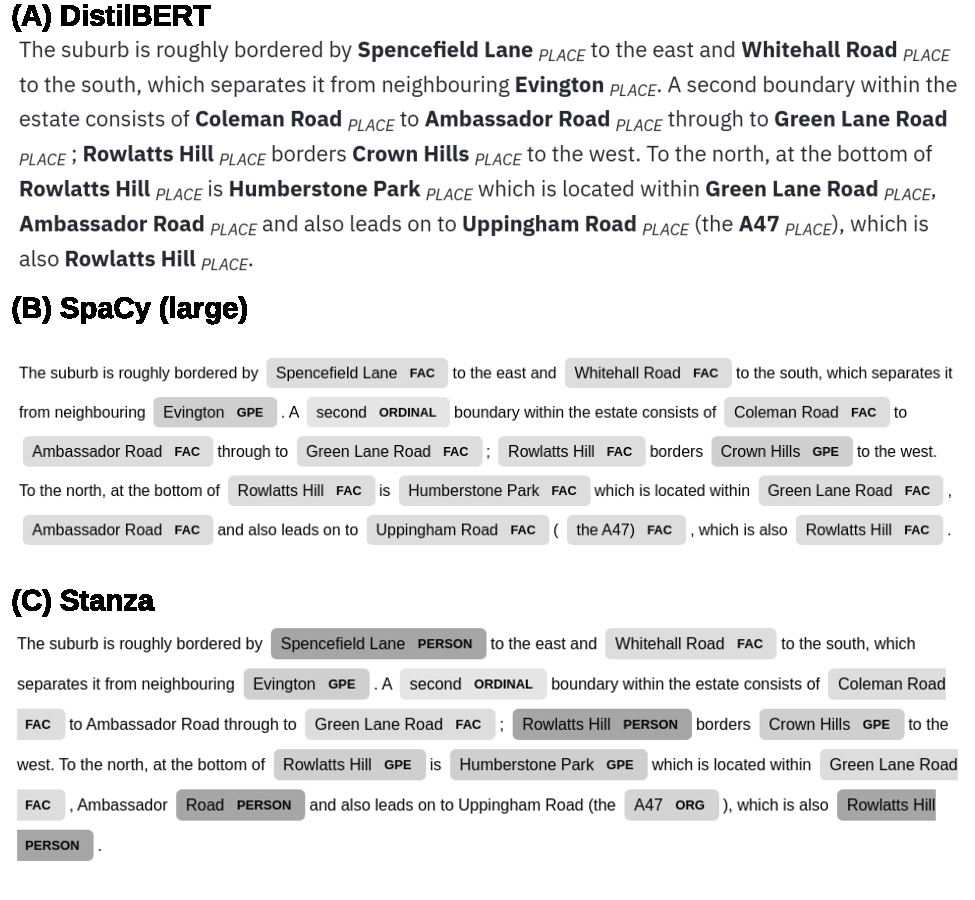
\includegraphics[width=.9\linewidth]{main_files/figure-latex/qual-1} 

}

\caption{Comparison of outputs between the best performing fine-tuned transformer model and the two best performing pre-built NER models.}\label{fig:qual}
\end{figure}

\begin{figure}[tb]

{\centering 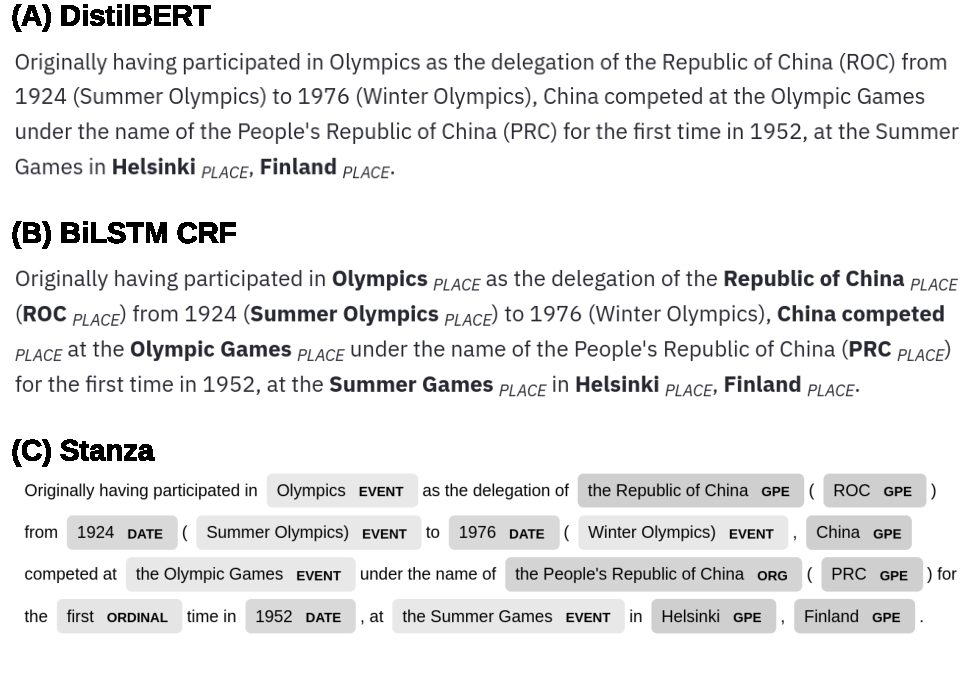
\includegraphics[width=.9\linewidth]{main_files/figure-latex/qual_china-1} 

}

\caption{Ability for trained model to distinguish between metonymic usage of place names.}\label{fig:qual_china}
\end{figure}

Figure \ref{fig:qual_china} demonstrates the ability for our DistilBERT
transformer model to accurately ignore entities that do not relate to
place names. This example paragraph only refers to a single geographic
location in text, the location of the 1952 Summer Games, in Helsinki,
Finland. While Stanza identifies a large number of GPE tags, they either
relate to China used in a metynomic sense, meaning the Chinese Olympic
team (`China competed'), or as a related geopolitical noun (`delegation
of ROC'), which is not considered to be a place name referring to a
geographic location in this context. Our model correctly infers the
single mention of a geographic place name based on the contextual
information, meaning a large amount of unrelated information is
excluded. Particularly, recognising and ignoring these nouns related to
place names is something that is noted as an issue in current geoparsing
systems \citep{gritta2020}. This figure also demonstrates the importance
of using a pre-trained model base for this task, as the BiLSTM CRF
performs poorly. It is likely that this issue stems from the limited
training data used, as the model is unable to learn more complex cases
where place names are less obvious (Figure \ref{fig:qual_china} (B)).
Using a pre-trained transformer enables the model to correctly identify
instances where proper nouns do not relate to place names, taking
information learned through its pre-training procedure.

\hypertarget{identified-place-names-from-wikipedia}{%
\subsection{Identified place names from
Wikipedia}\label{identified-place-names-from-wikipedia}}

\begin{table}
\caption{\label{tab:freq}Top and bottom named places by frequency, excluding any present in the GeoNames gazetter or mentioned less than 100 times.}

\centering
\fontsize{9}{11}\selectfont
\begin{tabular}[t]{lll}
\toprule
IDX & Place (DistilBERT) & Count\\
\midrule
70 & Great Western Railway & 236\\
77 & Ceredigion & 220\\
78 & West Riding of Yorkshire & 217\\
79 & East Lindsey & 217\\
83 & Midland Railway & 212\\
87 & London Underground & 195\\
... & ... & ...\\
176 & M4 & 108\\
180 & North Norfolk & 106\\
181 & M1 & 106\\
182 & Church of England & 106\\
191 & Hull & 104\\
199 & Great Northern Railway & 101\\
\bottomrule
\end{tabular}
\centering
\begin{tabular}[t]{lll}
\toprule
IDX & Place (SpaCy) & Count\\
\midrule
3 & the United Kingdom & 458\\
4 & Tyne & 353\\
5 & Ceredigion & 282\\
6 & the City of London & 211\\
7 & Methodist & 205\\
8 & the Metropolitan Borough of & 200\\
... & ... & ...\\
14 & France & 129\\
15 & Baptist & 127\\
16 & Sutherland & 119\\
17 & the City of & 116\\
18 & Richmondshire & 109\\
19 & Thameslink & 102\\
\bottomrule
\end{tabular}
\end{table}

Table \ref{tab:freq} gives an overview of the most common place names
identified by the DistilBERT model and the SpaCy model. Notably, the
SpaCy model appears to struggle with correctly aligning entities,
including `the' with `United Kingdom', and partially missing place names
containing `Tyne' (e.g.~`Tyne and Wear' or `River Tyne'). The DistilBERT
model also extracts around 6 times the number of place names compared
with SpaCy, reflected by the low recall noted above. One example where
the DistilBERT model appears confused is by giving the place name
`Church of England', this problem relates to the language used in
Wikipedia articles, when churches are described as a `Church of England
church', a nominal mention of a place rather than specific.

The total number of place names extracted from the Wikipedia summaries
by the \texttt{DistilBERT} model was 614,672, with 99,697 unique place
names. In total 62,178 unique place names were extracted that are not
found within the GeoNames gazetteer. These entities primarily exist as
granular names mentioned in single instances (e.g.~road names: Shady
Lane, Chapeltown Road), organisational names used in a place related
context (e.g.~describing locations along the Great Western Railway
route), and alternative names that are not captured by GeoNames. For
example, `M1' appears in GeoNames as `M1 Motorway'\footnote{\url{https://www.geonames.org/8714914/m1-motorway.html}}.
While the `M1 motorway' is used in Wikipedia articles, it is often also
referred to as just the `M1'.

\hypertarget{conclusion}{%
\section{Conclusion}\label{conclusion}}

Our paper demonstrates a new approach towards the extraction of place
names from text by building an NER model using data annotated with
geographic place names. This work aims to direct geographic NLP research
towards the use of models which move away from the generalisable
annotation schemes of pre-built NER solutions, to include task-specific,
relevant training data. Notably this differs from the perceived
generalisability of pre-built models used for general geoparsing. We
believe this is an important approach for geographic place name
extraction given geographic language differs greatly based on context
\citep{purves2018}, with contexts varying greatly based on the corpora
used for inference. This is demonstrated by the poor results observed in
previous work when applying pre-built NER solutions, which use training
data unrelated to the task-specific data they are being applied to
\citep{hu2019, karimzadeh2019}. \citet{wallgrun2018} recognise this
problem, developing GeoCorpora, a task-specific training dataset for
micro-blog geoparsing, notably describing increased issues with
annotation ambiguity compared with more traditional text-sources.
Additionally, recent work with transformer models, typically only built
to be generalisable, have considered moving from fully generalised
self-supervised training towards more dataset-specific models
(e.g.~TweetEval; \citet{barbieri2020}), with results that outperform
generalisable transformer models \citep{nguyen2020}.

Ultimately, the decision to produce a model explicitly designed to be
non-generalisable to other corpora may be considered a limitation of the
scope of this paper. We have demonstrated a best-case scenario where
time-frames allow for manual annotation of task-specific data. Future
research may consider the construction of a more generalisable place
name extraction model, which takes inspiration from the alternative
annotation scheme employed by our paper, allowing for use in general
purpose geoparsers.

Additionally, while our paper selects Wikipedia for place name
extraction, due to its large volume, ease of validation and data
retrieval, future work may consider the ability to apply our methodology
to other text sources. With suitable models constructed, using annotated
training data that is relevant to the corpus being considered, we expect
future work applied to other data sources may present the opportunity to
further contribute to place names that are absent from gazetteers, as
vernacular place names. We believe that given a suitable combination of
data sources, our methodology is the first step towards the construction
gazetteers from the bottom-up, directly taking place names from passive
contributions, without relying on pre-built datasets.

The recent development of pre-trained language models and their
suitability for fine-tuning in many tasks, including NER, presents a
method for the construction of accurate models that are task specific,
using relatively small labelled corpora\footnote{Compared with the
  Reuters corpus used for CoNLL03 for example} that defines entities
more suited to the task of place name extraction. The architecture in
our paper is more simplistic to implement than other attempts at similar
tasks \citep[e.g.][]{weissenbacher2019}, with most of the complexity
hidden within the transformer layers. This, combined with libraries that
abstract and implement state of the art models, provides a more
accessible approach for research in place name extraction, without
requiring a deep understanding of semantic rules, or the construction of
deep multi-layered models from the ground up.

Evaluation against pre-built NER models on Table \ref{tab:eval} shows
that performance for place name extraction is greatly improved,
particularly with respect to recall, a notable issue with past studies
\citep{hu2019, karimzadeh2019}. The construction of an NER model for the
task specific extraction of place names moves towards systems that
appropriately consider the geographic elements present in natural
language. The large number of place names that are absent from the
GeoNames gazetteer suggests that geoparsing and related work likely
misses a substantial amount of geographic information present in text.
The dataset produced through this work aims to assist with filling these
gaps, while the methodology described enables an approach that may be
mirrored and applied to further work on other data sources.

Finally, both `place' focussed annotation schemes describe the use of
`nominal' place related entities \citep{mani2010, pustejovsky2017}.
While out of the scope of our work, we would like to encourage the focus
on extracting this additional geographic information from text. Often in
language the use of these non-specific terms are used, for example `I
visited the shops', `York is a city', provide geographically specific
information. `The shops' with enough context may provide a specific
geographic location, and similarly the link between `York'
-\textgreater{} `city' could be explored \citep{couclelis2010}.

\hypertarget{data-and-codes-availability-statement}{%
\section*{Data and codes availability
statement}\label{data-and-codes-availability-statement}}
\addcontentsline{toc}{section}{Data and codes availability statement}

The data and codes that support the findings of this study are available
at the public FigShare link
(\url{https://doi.org/10.6084/m9.figshare.13415255.v1}). Instructions
for using the data and code are provided as a README within the FigShare
repository.

\hypertarget{disclosure-statement}{%
\section*{Disclosure statement}\label{disclosure-statement}}
\addcontentsline{toc}{section}{Disclosure statement}

No potential competing interest was reported by the authors.

\bibliographystyle{tfcad}
\bibliography{bib/main.bib}





\end{document}
